\documentclass[report.tex]{subfiles}

\externaldocument{report}

\begin{document}

\section{原理}

\wfig{all2}に今回作ったAMラジオの全体図を示す。
今回作ったAMラジオは、ラジオ回路と増幅回路からなる。

\begin{figure}[H]
	\centering
	\includegraphics[width=14cm]{fig/all2.pdf}
	\caption{全体}
	\label{fig:all2}
\end{figure}

\subsection{ラジオ回路}

\wfig{radio-circuit}にラジオ回路を示す。
ラジオ回路は、電波を受信するループアンテナ、受信した電波から取り出したい周波数を選択する同調回路、受信した電波から音声周波数を取り出す検波回路からなる。

\begin{figure}[H]
	\centering
	\includegraphics[width=7cm]{fig/radio.pdf}
	\caption{ラジオ回路}
	\label{fig:radio}
\end{figure}

\subsubsection{検波回路}

\begin{figure}[H]
	\centering
	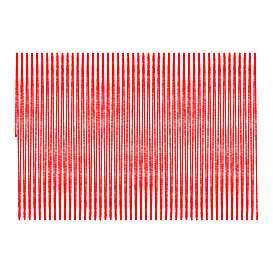
\includegraphics[width=7cm]{fig/5V.pdf}
	\caption{ラジオ回路}
	\label{fig:5V}
\end{figure}

\begin{figure}[H]
	\centering
	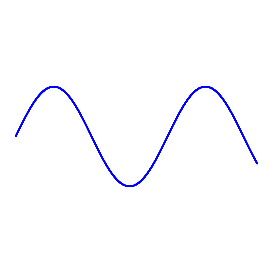
\includegraphics[width=7cm]{fig/3V.pdf}
	\caption{ラジオ回路}
	\label{fig:3V}
\end{figure}

\begin{figure}[H]
	\centering
	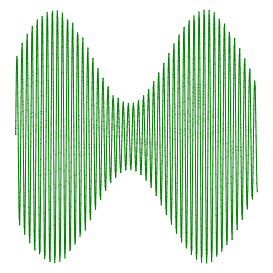
\includegraphics[width=7cm]{fig/Wave.pdf}
	\caption{ラジオ回路}
	\label{fig:wave}
\end{figure}

\begin{figure}[H]
	\centering
	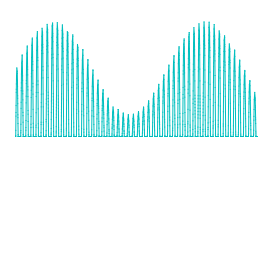
\includegraphics[width=7cm]{fig/diode.pdf}
	\caption{ラジオ回路}
	\label{fig:diode}
\end{figure}

\begin{figure}[H]
	\centering
	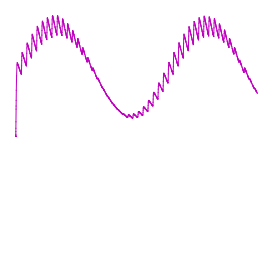
\includegraphics[width=7cm]{fig/capa.pdf}
	\caption{ラジオ回路}
	\label{fig:capa}
\end{figure}

\subsection{増幅回路}

\wfig{amplifier-circuit}に増幅回路を示す。
\wfig{amplifier-circuit}は、

\begin{figure}[H]
	\centering
	\includegraphics[width=15cm]{fig/amp.pdf}
	\caption{増幅回路}
	\label{fig:amplifier-circuit}
\end{figure}

\end{document}
